%---------------------------------------------------------------------------------------------------
%		use-cases.tex
%
%	This file contains the sections that describe typical use cases on which we can find the problem
% that will be studied in the master thesis.
%
%	Author: Andrea Meneghinello
% Version: 0.1
%	Table of changes:
%		06/03/2016 -> document definition
%---------------------------------------------------------------------------------------------------
\section[Typical use cases]{Typical uses cases}
\label{sec:problemSpace-useCases}
Nowadays more and more business companies\footnote{We refer to companies to which one that use
applications, hence excluding software-houses that produce applications.} use complex software systems
in their daily activities; from the customer care to internal administration. Typically these complex
applications are executed over proprietary hardware systems. This scenario is unfavourable for both
companies and software-houses that have to maintain the applications.

From the companies point of view, in order to keep those applications working, according
to the defined \ac{sla}, have to invest economic resources in qualified personnel and establish complex
administration processes. They can solve this problem through the adoption of one of the many existent
frameworks that allows \acs{it} process management. A well known one is \keyword{\ac{itil}}.
The framework, shown in Figure \ref{img:problemSpace-useCases-itilProcessModel}, defines general
best-practices in order to design and instantiate processes that permit a more coherent 
administration of \acs{it} departments and deployed applications. The processes that are relevant for
this problem belong to \ac{sda}. They are  \keyword{\ac{am}} and \keyword{\ac{cm}}. Both processes
focuses on planning and monitoring the effective provision of resources to support all the service
requirements \cite{availabilityCapacityProcesses}.

\begin{figure}
	\centering{}
	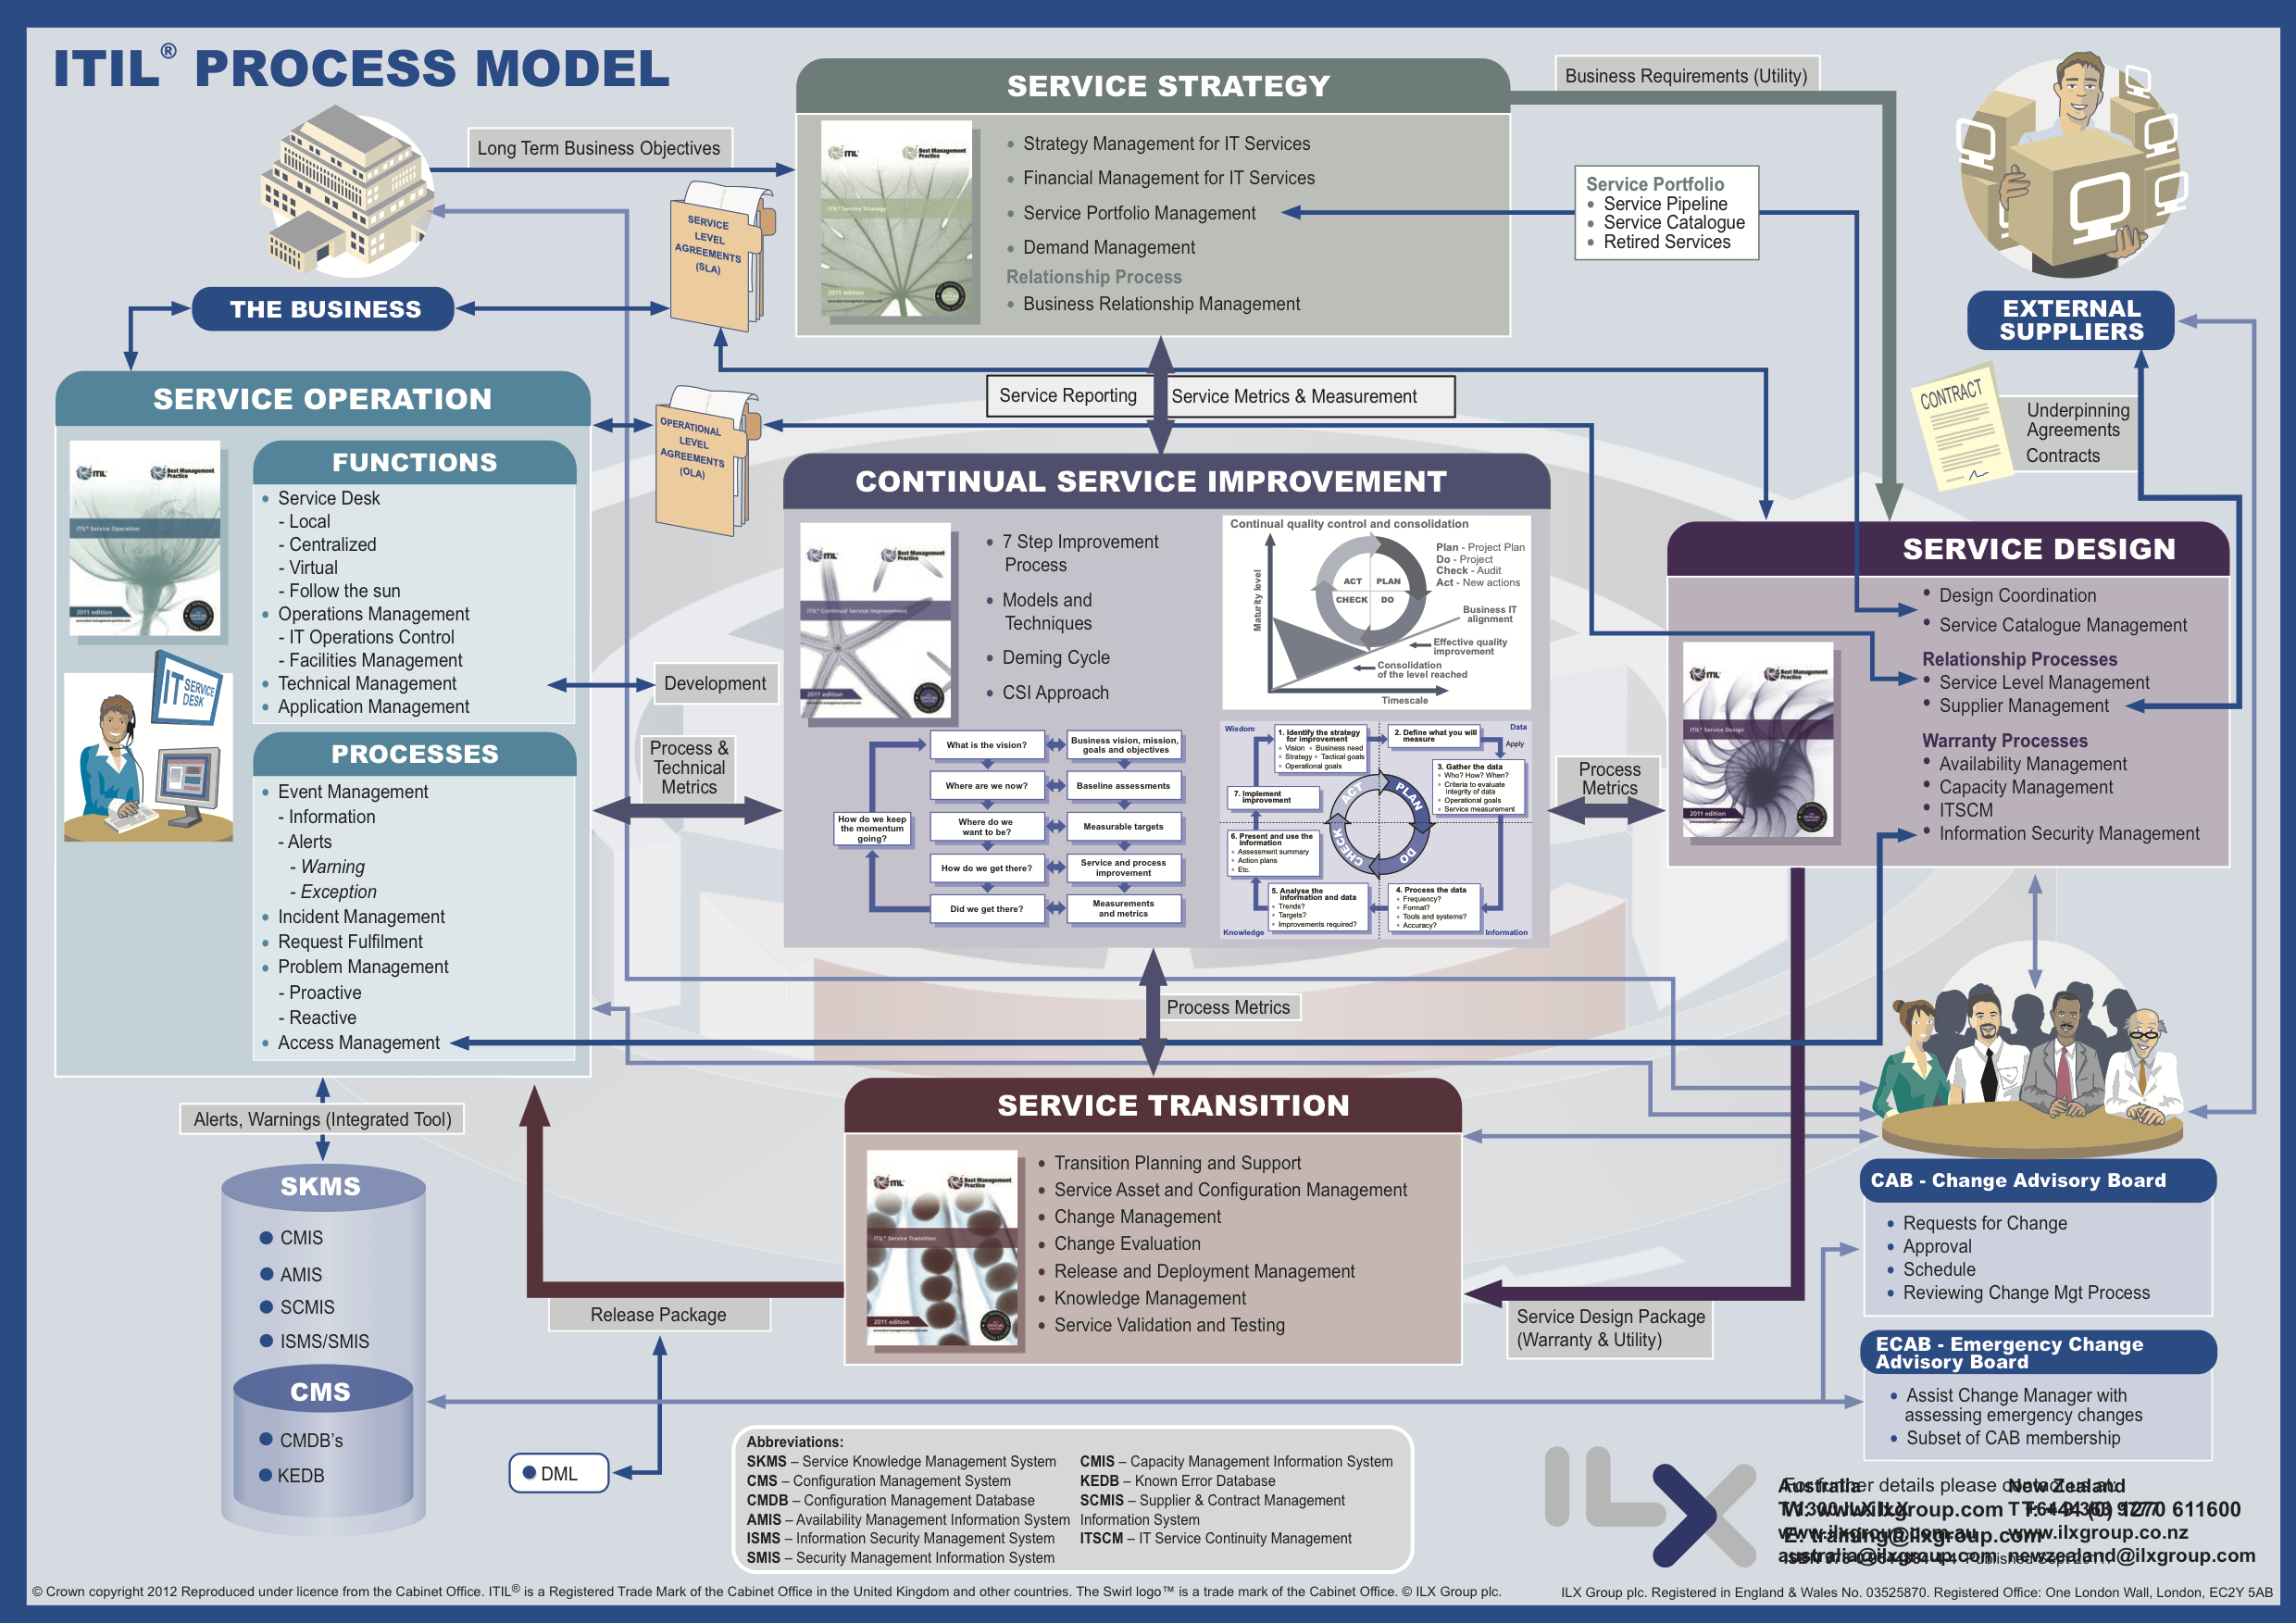
\includegraphics[width=0.8\textwidth]{chapters/problem/images/itil-map.png}
	\caption[\acs{itil} v3 process model]{A bird's eye view of the processes defined by the \acf{itil} 
		framework. Their main purpose is to manage software's life-cycle in large business companies
		\cite{itilProcessModel}.}
	\label{img:problemSpace-useCases-itilProcessModel}
\end{figure}

On the other hand software-houses have to face with different runtime environments (both in term of
hardware and software configurations) which makes the \glossaryPlr{deployment-process} more difficult.
Another problem is represented by unavoidable bug errors that are present in every application. Here
bugs are not only due to development errors but they can be also due to the runtime environment itself.
Thus developers waste a lot of time only to replicate the execution environments, stealing it from
more profitable activities. Finally when the solution is found they have to visit the client to fix
the bugs in loco (if remote assistance is not possible).

Another use case is the following: software-houses may want to make their software available online
and always up-to-date. End users should be able to use it anywhere and using any type of device without
any installation process. In addiction they do not have to care about updating that software.

Companies can follow general best-practices to solve the problem. In addiction, many of them have
understood, very well, the benefit of delegating hardware management to cloud providers (see section
\ref{sec:problemSpace-capexOpex}). Unfortunately, we cannot assert the same things for software-houses.

In the last decade, cloud computing model have become a more reliable infrastructure supplier, so companies 
started to earn outsourcing the hardware management. Nevertheless software engineers have to face again
with the construction and the configuration of complex scalable environments, stealing time from developing
activities. As a consequence they ask for more automation in building work environments  (execution,
development and test) so they can focus more on development activities.

Nowadays cloud computing is able not only to offer them unlimited provision of hardware but also
the generation of dynamic work environments. In order to understand how it is possible we must first
interpret what really is cloud computing and why it is able to help both business companies and
software-houses.